\documentclass[10pt,twocolumn]{article}
\usepackage[margin=0.7in]{geometry}
\usepackage[T1]{fontenc}
\usepackage{lmodern}
\usepackage{microtype}
\usepackage{graphicx}
\usepackage{enumitem}
\usepackage[hidelinks]{hyperref}
\setlist{nosep,leftmargin=*}
\setlength{\columnsep}{0.25in}
\setlength{\textfloatsep}{8pt}
\setlength{\abovecaptionskip}{3pt}
\setlength{\parskip}{2pt}
\makeatletter
\renewcommand\section{\@startsection{section}{1}{\z@}{6pt}{3pt}{\normalfont\large\bfseries}}
\renewcommand\paragraph{\@startsection{paragraph}{4}{\z@}{3pt}{-0.5em}{\normalfont\bfseries}}
\makeatother
\newcommand{\num}[1]{\textbf{#1}}

\title{\vspace{-0.65in}\textbf{Repository Intelligence Layer: Mid-Term Report}\\[2pt]
\large Does the quality of a retriever's training data reach coding-agent success?}
\author{Sukhraj Singh\\ \small 2025202009 \and Neill Rawani\\ \small 2025202027 \and
Chaitanya Shah\\ \small 2025202033}
\date{\vspace{-6pt}IIIT Hyderabad}

\begin{document}
\maketitle
\vspace{-0.4in}

% =============================================================================================
\section{Problem}

Coding agents work inside a fixed context window, while a real repository is many times larger.
Before an agent can fix an issue, something has to decide which code it reads. When that choice is
poor, the agent spends tokens and time exploring irrelevant files, or never sees the code it has to
change. We build the \emph{Repository Intelligence Layer} (RIL): given an issue, it returns a small,
ranked set of code units, so that the agent works only on the part of the repository that matters.

\paragraph{The system.} RIL indexes a Python repository at function level: every top-level function,
method and class is a unit, plus one unit per file for module-level code. Three signals score units
against the issue text: \emph{BM25}, a lexical match on words and identifiers; a \emph{dense
encoder}, semantic similarity from a code embedding model; and a \emph{code graph} of calls, imports,
inheritance and containment, which can pull in structurally related units. The signals are fused by
reciprocal rank fusion, and the top units are packed into the agent's context under a token budget.
Every stage is profiled for latency (p50/p95/p99).

\paragraph{What differs from current practice.} Retrievers for code agents are usually trained with
conventional data-cleaning choices and judged on retrieval metrics alone. We make the training data
the experimental variable and follow its effect through retrieval quality to whether the agent
actually fixes the bug, with the agent held fixed. Our literature audit did not identify a study
that evaluates this chain end to end. We also extend the code graph with links to tests and
configuration files: no published graph schema has them, although the benchmark's Level-3 task
scores exactly that context.

\paragraph{Study.} Training pairs for repository retrieval are mined from pull requests, with the
issue text as the query and the edited functions as positives. They are noisy: an edited function is
not always the one the issue is about. We compare four ways of handling that noise, each training the
same encoder for the same number of optimizer updates (\emph{matched optimization budgets}):
\textsc{Raw} (all pairs); \textsc{Filter} (drop pairs whose positive a separately pretrained
retriever ranks below $K$, the K-rank signal of SweRank); \textsc{Weight} (keep all pairs,
down-weighted by the same signal); and \textsc{Curriculum} (easy pairs first).

\paragraph{Questions.} \textbf{RQ1:} which signals (dense, +BM25, +graph, all three) contribute,
and at what latency cost? This fixes the stack the other questions hold constant. \textbf{RQ2:} how
does supervision quality change retrieval quality at matched budgets? Our hypothesis is that
\textsc{Filter} and \textsc{Weight} beat \textsc{Raw} at equal updates; the early pilots below do not
show this yet. \textbf{RQ3:} does a better retriever raise the agent's resolved rate? Each RQ2
retriever is plugged into one fixed agent (same model, temperature, seed and issues). For every
failure we record whether the file of the reference fix was retrieved. This separates retrieval
failures from reasoning failures, so a null result can still be explained.

% =============================================================================================
\section{Progress}

\paragraph{1. Evaluation harness.} Benchmark loader (CORE-Bench), metrics and function-level scoring
are built. Every choice is tuned on development repositories (SWE-bench Pro and Live), SWE-bench
Verified is kept for one final look, and intervals are bootstrapped over repositories.
\emph{Finding:} our BM25 reproduces the published baseline to the printed decimal (Verified L2
nDCG@10 \num{11.94} vs.\ 11.9; L3 Recall@100 \num{33.89} vs.\ 33.9), so our numbers are directly
comparable to the literature.

\paragraph{2. Leakage and contamination control.} A held-out list of 605 benchmark repositories
(plus 169 from a second benchmark), with renamed repositories resolved, filters every training pool
at repository level. \emph{Findings:} the public training pool used by recent work contains
\num{89 benchmark repositories (14.1\% of its pull requests)}; we removed them. In a large public code
corpus, \num{13.7\%} of the test repositories' functions appear verbatim, but only \num{8.9\%} of the
functions the reference fixes edit. Memorisation therefore touches the surrounding code more than the
code that has to change.

\paragraph{3. Parser and code graph.} Function-level units with a frozen schema, our own static call
resolver, and typed edges that carry a status (resolved, ambiguous, external, unresolved). Rebuilds
are byte-identical (django: 35,860 units). We added an \emph{incremental update} that re-reads only
the files a commit changes and the files that depend on them. \emph{Finding:} on 100 real commits of
five repositories, the incremental graph was \num{identical to a full rebuild every time} and up to
\num{9.6$\times$ faster} (django: 29.2\,s $\to$ 3.0\,s per commit; Fig.~\ref{fig:incremental}). The
equality check also exposed a cache in the resolver that made some edges depend on the order in which
files were processed; it is fixed.

\begin{figure}[t]
\centering
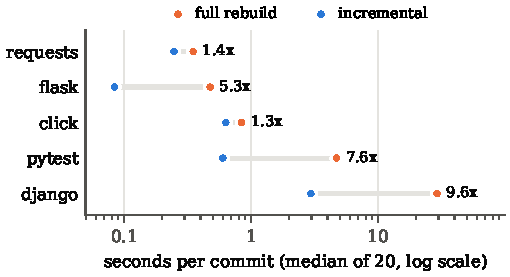
\includegraphics[width=\columnwidth]{fig_incremental.pdf}
\caption{Graph update cost per commit, incremental vs.\ full rebuild (median of 20 commits; labels
give the median per-commit speedup). Every update equals the full rebuild.}
\label{fig:incremental}
\end{figure}

\paragraph{4. The graph as a retrieval signal.} \emph{Finding:} on top of a fused BM25 and dense
first stage, expanding along typed graph edges is no better than adding other functions from the same
file (L3 Recall@100 \num{$-2.7$} [$-6.0$, $+0.8$]). Tests do matter: test functions are \num{20.5\%}
of the relevant units in L3 and \num{44\%} of those outside the issue's main files. The planned test
edges target exactly these.

\paragraph{5. Lexical signal.} Identifier splitting (\texttt{get\_adapter} $\to$ \emph{get},
\emph{adapter}) and per-field weights. \emph{Finding} (local pilot: 2,649 queries, each a function's
docstring summary, over five repositories, with all docstrings removed from the index): MRR rises from
\num{18.7 to 27.6} ($+8.9$ [$+6.9$, $+10.5$]), and to \num{31.9} with a higher weight on the function
name. Query latency is unchanged (at most 1.3\,ms p99 over 41k units; Fig.~\ref{fig:bm25}). Docstrings
share words with function names more than bug reports do, so this is an upper bound until the
benchmark runs.

\begin{figure}[t]
\centering
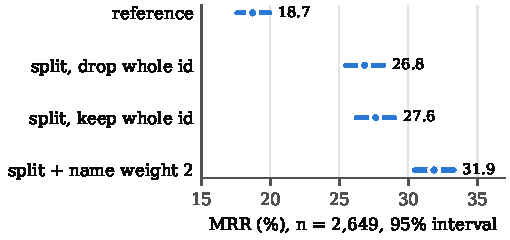
\includegraphics[width=\columnwidth]{fig_bm25.pdf}
\caption{BM25 variants on docstring-to-function retrieval (five repositories, docstrings removed
from the index; exploratory pilot).}
\label{fig:bm25}
\end{figure}

\paragraph{6. Dense encoders.} CodeRankEmbed and Qwen3-Embedding-0.6B, used without fine-tuning
over an exact index. \emph{Finding:} the larger model's gain after fusion is small and not
significant ($+1.9$ L2, $+3.4$ L3; both intervals include 0), while its query latency is
\num{2.5--3.7$\times$} higher (GPU 18 vs.\ 45\,ms; CPU 0.41 vs.\ 1.53\,s). It also cannot be
fine-tuned on an 11\,GB GPU. CodeRankEmbed is therefore the base encoder.

\paragraph{7. Training stack and pilots.} Multi-positive contrastive training with negatives from
the same repository. The arms differ only through filter, weight and ordering hooks, and a test
confirms that everything else is bit-identical. \emph{Findings:} \textsc{Raw} training lifts L2
nDCG@10 by \num{$+10.5$} [$+8.3$, $+12.7$] within 100 updates, then stays flat up to 2,000. At pilot
scale no \textsc{Filter}, \textsc{Weight} or \textsc{Curriculum} setting beats \textsc{Raw} (strict
filters are 0.6--1.6 points below). A likely reason: the public pool already looks filtered by a
retriever. \num{0 of 160} sampled training directories lack a positive in that retriever's top 10,
against \num{19.3\%} on benchmark data that was never filtered. So ``raw'' is not raw.

% =============================================================================================
\section{Risks}

\begin{itemize}
  \item \textbf{A pre-filtered training pool.} If the public pool was already selected by a
  retriever, \textsc{Raw} and \textsc{Filter} differ less than intended and the RQ2 effects shrink.
  This is why we are building our own unfiltered set mined from pull requests.
  \item \textbf{Small effects against benchmark size.} Pilot differences between arms are at most
  1.6 points. On SWE-bench Verified (432 issues), a resolved-rate test detects differences of
  roughly 4.5--7.75 points or more, so a real but small RQ3 effect may not be distinguishable.
  \item \textbf{A static call resolver.} Dynamic calls stay unresolved, and the cache bug showed that
  subtle errors can hide in edges. Weak edges may explain the graph's null result as much as the idea
  does.
  \item \textbf{Proxy measurements.} Local pilots (docstring queries, short training runs) can
  overstate or understate effects on real issue text.
  \item \textbf{Benchmark labels.} Level-3 labels are judged by a language model, Level-2 positives
  include import blocks, and mapping benchmark chunks to our function units involves choices; some
  orderings flip between the two ways of reading the gold labels.
  \item \textbf{Contamination.} Pretraining exposure inflates absolute scores. It is identical across
  arms, so comparisons hold, but absolute numbers are not capability claims.
  \item \textbf{Compute.} Benchmark-scale encoding and training run on a shared cluster. Queueing and
  the memory of the available GPUs limit model choice and the number of runs.
\end{itemize}

% =============================================================================================
\section{Plan}

\begin{itemize}
  \item Tune and freeze the retrieval stack (BM25, encoder, fusion, rerank); RQ1 ablation with
  latency.
  \item Build the unfiltered training set; train four arms $\times$ three seeds at matched budgets
  (RQ2).
  \item Go/no-go: at least two retrievers with a measurable retrieval difference.
  \item Fixed-agent paired runs with the failure breakdown (RQ3); test and config edges for L3.
  \item Analysis and final report. If RQ3 is cut, the fallback is RQ1 + RQ2 + the latency study.
\end{itemize}

\end{document}
